\documentclass[11pt]{article}

\usepackage[margin=1.15in]{geometry}
\usepackage{amsmath}
\usepackage{booktabs}
\usepackage{graphicx}
\usepackage{microtype}
\usepackage[round]{natbib}
\usepackage[hidelinks]{hyperref}
\usepackage{caption}
\captionsetup{font=small, labelfont=bf}

\newcommand{\pkg}[1]{\texttt{#1}}

\title{Elections on measured stakes:\\
welfare tracking and platform competition\\
with microsimulated household impacts}
\author{Max Ghenis\thanks{max@maxghenis.com. Code, data artifact, and every
number's regeneration script: \url{https://github.com/MaxGhenis/democrasim}.
The author co-founded PolicyEngine, whose open models and data this
personal project uses.}}
\date{July 12, 2026}

\begin{document}
\maketitle

\begin{abstract}
\noindent
Does plurality voting select the policy a stated social welfare function
prefers when voters misperceive their own stakes? I study the question in
a simulation whose inputs are measured and whose behavioral layers are
explicit modeling choices: the electorate is 120{,}408 voting-age adults
from certified, population-calibrated US microdata; the two platforms are
actual encoded tax reforms with opposite incidence, budget-matched within
3\%; each voter's stake is the tax engine's computed change in their
household's net income, closed by a labeled financing rule; and
perception --- truth plus Gaussian noise plus optional shared bias --- is
the headline assumption. For plurality the model admits an analytic
normal approximation at any electorate size, exact in the
large-population limit. Measured stakes are two-cliffed: net of financing, three-quarters of
adults hold under \$25 a year while over a fifth hold more than \$500,
and this structure overturns standard toy-model intuitions.
Tracking is non-monotone in accuracy: at perfect information the outcome is
decided by the \emph{sign} of a \$4.10-per-adult financing residual --- a
welfare-irrelevant quantity --- while moderate noise (\(\sigma \approx
\$50\)--\$2{,}000) restores near-certain tracking by turning the
trivial-stakes mass into canceling coin flips. Tracking thresholds are
electorate-size statements that collapse toward 0.5 accuracy as \(n\)
grows, while the expected-vote-share crossing behind the failure ceiling
does not move with \(n\). And shared misperception of
\(\approx\$221\) per voter per year flips elections that \$1{,}000 of
independent noise cannot move. Making the platforms choices reverses the
information verdict: when two candidates --- households from the data,
each valuing their own stake and society's equally-distributed-equivalent
income change on one dollar scale --- pick positions in the space the
measured incidence vectors span, perfect information becomes an
undercutting force that drives every pure Nash equilibrium to the status
quo, the welfare optimum available, while noise lets both self-serving
programs escalate to full intensity and erodes the electoral advantage of
the broad-constituency program over the narrow one. Giving voters the
same mixed motives restores order cheaply: 3.8\% of utility weight on
society cures the knife-edge, a 10\% informed-sociotropic minority
disciplines purely selfish candidates back to the status quo at every
noise level (traversing a cycling regime around 2--5\% shares where
the pure-equilibrium set can be empty), and the residual distortion is
value pluralism --- fully
informed sociotropic voters split when their inequality aversions
disagree. With the status quo votable as a third ballot option, every
rule tested --- plurality, approval, score, STAR, instant runoff ---
tracks perfectly at perfect information: the knife-edge was ballot
design, not aggregation. The exception prices a convention: under
strict approval the status quo itself can never be approved, one
program's beneficiaries elect it unopposed, and the threshold
instruction alone swings perfect-information tracking from 0\% to
100\% in an electorate where three in four voters are near-indifferent;
under noise the ordering reverses --- approval most robust, plurality
worst --- and every gap between rules stays smaller than what the
agenda decides. And on a continuous redistribution axis --- every
bracket rate up to ten points higher, revenue returned as a \$4{,}809
per-adult transfer at full intensity, 68.6\% of households gaining ---
demand for policy inflates with the reciprocal of belief in its reach
(a voter wanting half the achievable inequality reduction who believes
policy half as effective demands the entire axis), two-candidate
competition enacts the median belief rather than the canceling mean,
and a purely self-interested electorate enacts the maximum at every
noise level; moderation there comes from values or beliefs, not
stakes. The mechanisms are classical; the contribution is
dollar-denominated calibration on measured microdata, a reusable
open-source harness, and a direct path to replacing the perception
assumption with survey estimates.
\end{abstract}

\section{Introduction}

A large literature asks when majority voting aggregates dispersed
information or dispersed interests into good collective choices. The
Condorcet jury theorem gives the optimistic benchmark: homogeneous stakes
and independent errors let even barely-informed majorities decide almost
perfectly \citep{condorcet1785}. Its known failure modes are equally
classical: correlated errors break the aggregation \citep{ladha1992},
the crux of the miracle-of-aggregation debate
\citep{page1992, caplan2007}; intense minorities lose to
indifferent majorities under one-person-one-vote \citep{dahl1956};
rationally ignorant voters may economize on information
\citep{downs1957}, and less-informed voters may strategically abstain in
common-value settings \citep{feddersen1996} --- a distinct mechanism from
the private-stake indifference abstention modeled here; and probabilistic-voting
models tie what elections aggregate to the responsiveness of vote
probabilities \citep{coughlin1981, lindbeck1987}.

What this paper adds is not a new mechanism but a new input quality.
Simulation exercises in this tradition typically invent the key
quantity --- the distribution of what voters stand to gain or lose ---
and the invented distributions drive the conclusions. Here the inputs are measured and the behavioral layers are explicitly
labeled. The electorate is population-calibrated microdata; the platforms are
actual encoded reforms; the stakes are computed by a tax-benefit
microsimulation engine, household by household, including interactions
across programs. On these inputs, several toy-model conclusions reverse,
and the surviving ones acquire dollar denominations: how many dollars of
noise elections tolerate (thousands), how many dollars of shared bias they
do not (about \$221 per voter per year), and how many dollars of stake the
decisive voting bloc holds at perfect information (\$4.10 per adult per
year, net of financing).

Five fixed-platform results come first. First, measured stakes are
nothing like the homogeneous or Gaussian stakes of standard toys: 76\% of
adults have approximately \$0 at stake gross of financing, while a fifth
hold stakes above \$500 (Section~\ref{sec:stakes}). Second, welfare
tracking is non-monotone in perception accuracy, and its failure at
perfect information is a knife-edge with a precise anatomy: the outcome
becomes \emph{welfare-independent}, set by the sign of the residual cost
gap between the two policies (Section~\ref{sec:knife}). Third, every
tracking threshold is an electorate-size statement; a closed form places
the Monte Carlo results on the full ladder from 101 voters to the
large-population limit (Section~\ref{sec:n}). Fourth, elections in this
environment are robust to large independent misperception and fragile to
small shared misperception (Section~\ref{sec:bias}). Fifth,
moment-matched Gaussian comparators --- even preserving impact--income
covariance --- reproduce none of this structure, so calibrating stake
\emph{shape} matters more than matching moments (Section~\ref{sec:toys}).

Two further layers then make behavior endogenous, on both sides of the
ballot. Platforms become choices: two policy-motivated candidates
\citep{wittman1983, calvert1985} --- households drawn from the data, in
the citizen-candidate spirit \citep{osborne1996, besley1997} --- pick
positions in the two-dimensional space the measured incidence vectors
span, and every pure Nash equilibrium is computed exactly
(Section~\ref{sec:strategic}). And voters get the same utility family
the candidates carry: a selfish weight on their own perceived stake and
a societal weight on the policy's equally-distributed-equivalent income
change \citep{atkinson1970}, the sociotropic motive of
\citet{kinder1981} and the altruistic-voting calculus of
\citet{edlin2007} in dollar form, with mixtures of types heterogeneous
in weights, inequality aversion, and information quality
(Section~\ref{sec:preferences}). The two layers interact: the
information conditions under which elections grade fixed policies well
are close to the opposite of those under which they discipline the
policies candidates offer.

Two extensions widen what voters choose among. Putting the status quo
on the ballot as a third option dissolves the perfect-information
knife-edge under every voting rule tested --- the two-option failure
was ballot design, not a plurality pathology --- while approval
voting's threshold convention alone swings the perfect-information
outcome between 0\% and 100\%, noise reverses the rule ordering with
approval most robust and plurality worst, and every gap between rules
stays smaller than what the agenda decides (Section~\ref{sec:rules}).
And replacing the policy pair with a continuous redistribution axis ---
every bracket rate up to ten points higher, revenue returned per
adult --- turns demand for policy into a derived quantity: voters who
understate policy's reach demand more of it, reciprocally;
two-candidate competition enacts the median belief rather than the
canceling mean; and a purely self-interested electorate on measured
incidence enacts the maximum at every noise level, the demand side of
\citet{meltzer1981} in operation (Section~\ref{sec:axis}).

The exercise is a thought experiment about one mechanism: self-interested
voting on misperceived, engine-computed household impacts. It is not
political science and predicts no elections; real voters weigh values,
identity, and information far beyond their own net income
\citep{bartels2005, stantcheva2021}. Platforms are labeled generically
throughout.

\section{Model}\label{sec:model}

\paragraph{Electorate.} Each voter \(i\) is a voting-age adult carrying
their household's true impact \(\delta_{ij}\) (dollars per year) under each
policy \(j \in \{A, B\}\), a survey weight, baseline household net income,
and the household's adult count \(a_i\). Voting is per adult; welfare
counts each household's dollars once (contributions divide by \(a_i\)).

\paragraph{Financing.} Engine impacts are gross: a tax cut shows only
winners. The headline specification levies each policy's total cost equally
per adult, making both policies budget-neutral by construction;
a proportional-to-income levy and the unfinanced gross case are stress
tests. Net stakes and the margin \(m_i = \delta_{iA} - \delta_{iB}\) are
defined after financing.

\paragraph{Welfare.} An isoelastic social welfare function over household
net income (\(\eta = 1\), incomes floored at \$1{,}000) ranks the two
policies; ``tracked'' means the election selects the \emph{ballot-best}
policy, the higher-ranked of the two. Under this metric both financed
policies score below the status quo, which plurality does not offer; Section~\ref{sec:knife} returns to this.

\paragraph{Perception and voting.} Voter \(i\) perceives
\(\hat\delta_{ij} = \delta_{ij} + b_j + \varepsilon_{ij}\) with
\(\varepsilon_{ij} \sim N(0, \sigma^2)\) i.i.d.\ across voters and
policies, and \(b_j\) a shared bias. Under plurality with
abstention at exact perceived indifference, voter \(i\) votes for \(A\)
with probability
\begin{equation}
p_i(\sigma, b) \;=\; \Phi\!\left(\frac{m_i - (b_B - b_A)}{\sigma\sqrt{2}}\right)
\qquad (\sigma > 0),
\label{eq:probit}
\end{equation}
while at \(\sigma = 0\) the vote is deterministic: \(A\) if the shifted
margin is positive, \(B\) if negative, abstention if exactly zero.
The implementation also supports multiplicative attenuation of
\(m_i\), fixed to 1 throughout this paper. An election of \(n\) voters
sampled with probability proportional to weight then reduces to a
multinomial over (\(A\), \(B\), abstain) with
population-weighted mean probabilities \((\bar p_A, \bar p_B, \bar p_0)\).
With \(g = \bar p_A - \bar p_B\), the probability that \(A\) wins is
\(\Phi\!\big(ng / \sqrt{n(\bar p_A + \bar p_B - g^2)}\big)\) by the normal
approximation, degenerating to a step function of \(g\) as
\(n \to \infty\). All plurality results use this normal approximation (exact in the
large-population limit) or Monte Carlo simulation that matches it;
approval voting and instant-runoff variants are simulated directly, and
with two policies instant-runoff coincides with plurality absent exact
ties.

\section{Data and calibration}\label{sec:data}

The electorate comes from PolicyEngine's certified, population-calibrated
Populace microdata for the United States (57{,}240 households; 120{,}408
adults representing 268 million), scored with \pkg{policyengine-us} 1.764.6
for policy year 2026. Policy A raises the federal Child Tax Credit base
amount from \$2{,}200 to \$3{,}200; Policy B caps the top two marginal
income tax rates at 34\%. The engine scores them at \$39.1B and \$38.0B a
year of household net income change (model totals including state-tax
interactions, not budget scores) --- within 2.9\%, so neither platform is
simply the larger transfer. Incidence is opposite: 9.9\% of Policy A's
dollars reach the top income decile versus 99.7\% of Policy B's.

The committed data artifact carries full provenance (engine versions,
certified dataset revision and hash, reform parameter dictionaries) and
passes builder validations that reconcile every extracted quantity against
the engine's own weighted aggregates (worst relative discrepancy
\(10^{-16}\)). Regression tests pin the artifact facts the results below
depend on --- most fragilely, the sign of the cost gap --- so a future data
rebuild cannot silently invert them.

\section{Fixed platforms: elections as graders}\label{sec:fixed}

\subsection{Measured stakes are two-cliffed}\label{sec:stakes}

\begin{figure}[t]
\centering
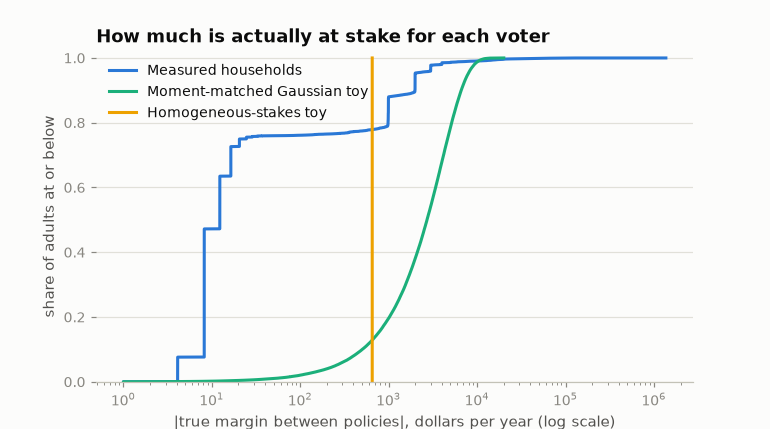
\includegraphics[width=.86\linewidth]{figures/margin_distribution.png}
\caption{Weighted cumulative distribution of \(|m_i|\), the true margin
between the two policies per adult, net of per-capita financing. Measured
households form a staircase --- 47\% of adults within \$10, 75.5\% within
\$25, driven by the \$4.10-per-adult difference in the two policies'
levies --- with a high-stakes tail. The two synthetic comparators used by
toy models lack this structure.}
\label{fig:margins}
\end{figure}

Gross of financing, 76\% of adults see approximately \$0 from both
policies; Policy A's gains arrive in per-child quanta of about \$1{,}000
for the 20\% of households with eligible children. Financing hands the
untouched majority a small signed stake: the two levies differ by \$4.10
per adult per year, so 75.5\% of adults hold margins under \$25 while
19.9\% (all in households with children) hold pro-\(A\) margins above
\$500 and 2.6\% hold pro-\(B\) margins below \(-\$500\)
(Figure~\ref{fig:margins}). The weighted mean absolute margin, \$652,
describes almost nobody.

\subsection{Non-monotone tracking and the welfare-independence knife-edge}
\label{sec:knife}

\begin{figure}[t]
\centering

\includegraphics[width=.86\linewidth]{figures/accuracy_curve.png}
\caption{Share of 10{,}001-voter elections electing the ballot-best policy
(240 elections per point; Wilson 95\% bands), against mean ranking
accuracy --- the probability a voter correctly ranks the two policies for
their own household. The homogeneous toy is the Condorcet jury theorem;
the measured curve fails at \emph{both} ends.}
\label{fig:accuracy}
\end{figure}

At 10{,}001 sampled voters, tracking is essentially perfect for noise
\(\sigma\) between about \$50 and \$2{,}000 (every estimate 1.000, Wilson
lower bounds 0.984) and collapses at both extremes
(Figure~\ref{fig:accuracy}). The high-noise decay is ordinary. The
perfect-information failure is not: at \(\sigma = 0\), 78.7\% of adults
strictly prefer Policy B --- including the 76\% of all adults untouched
by either reform, whose entire stake is the \$4.10 levy gap --- and
plurality elects \(B\) in every election, the opposite of the
welfare ranking.

Table~\ref{tab:knife} dissects the knife-edge. The direction is set
entirely by the sign of the residual cost gap: rescaling Policy B to cost
3\% \emph{more} than A flips perfect-information tracking from 0\% to
100\% with the welfare ranking unchanged. The mass only rules while it
votes: exact parity or unfinanced gross stakes leave it exactly
indifferent, it abstains (turnout 24\%), and tracking holds from accuracy
\(\approx 0.59\) through perfect information. A behavioral \$25
indifference band does the same; a \$10 band does not, because multi-adult
households' levy margins exceed it. Approval voting reaches the same
outcome through self-silencing --- voters who perceive both policies as
net losses approve neither --- though under the three-option ranking the
welfare metric itself induces (status quo first), a winner elected on
23\% turnout is still a welfare-reducing enactment; approval's property here is the
filter, not welfare optimality.

\begin{table}[t]
\centering
\small
\begin{tabular}{lccl}
\toprule
Variant (perfect information) & Tracked & Turnout & Decisive margin \\
\midrule
Per-capita financing (headline) & 0\% & 100\% & \(-\$4.10\) levy gap \\
Proportional financing & 0\% & 99.8\% & same sign, income-scaled \\
Sign-flip counterfactual (B costs $+3\%$) & 100\% & 100\% & \(+\$4.38\) levy gap \\
Exact-parity counterfactual & 100\% & 24\% & \$0 (mass abstains) \\
Gross stakes (no financing) & 100\% & 24\% & \$0 (mass abstains) \\
Abstention band \$10 & 0\% & 53\% & multi-adult margins survive \\
Abstention band \$25 & 100\% & 24\% & staircase silenced \\
Approval voting & 100\% & 23\% & mass approves neither \\
\bottomrule
\end{tabular}
\caption{The perfect-information knife-edge under stress. Counterfactual
rows are synthetic rescalings of Policy B's gross impacts, labeled as such
in the regeneration scripts.}
\label{tab:knife}
\end{table}

Perfect information therefore does not make elections anti-track welfare;
it makes them \emph{welfare-independent}, delegating the outcome to
whichever side of an arbitrary residual the no-stakes bloc shares. Between
the extremes, moderate misperception helps: noise converts four-dollar
margins into fair coins that cancel, and the informed high-stakes minority
decides. This parallels the logic of probabilistic-voting models
\citep{coughlin1981, lindbeck1987}: idiosyncratic noise makes plurality
weight stakes, and vanishing noise reverts it to counting heads --- here
traversed numerically on measured stakes.

\subsection{Thresholds are electorate-size statements}\label{sec:n}

\begin{figure}[t]
\centering
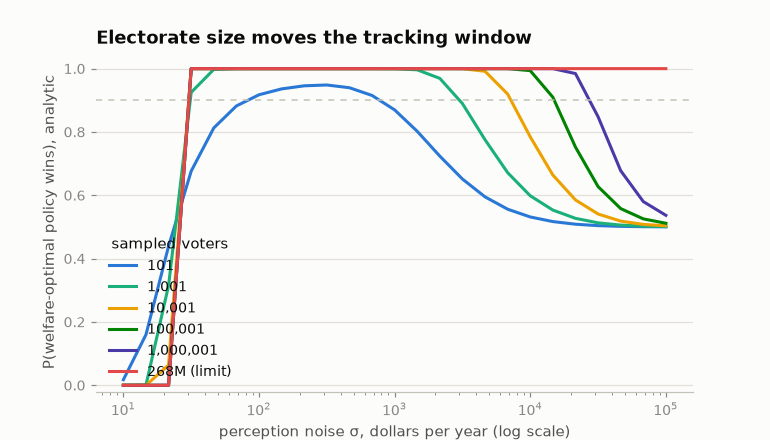
\includegraphics[width=.86\linewidth]{figures/n_sensitivity.png}
\caption{Analytic tracking probability by electorate size, per-capita
financing, against noise \(\sigma\) (log dollars). On this axis the
knife-edge is the fixed left wall near \(\sigma \approx \$25\); the
right slope, where noise finally drowns the high-stakes signal, is the
jury-theorem edge that moves with \(n\).}
\label{fig:n}
\end{figure}

The accuracy band in which tracking exceeds 90\% runs from 0.598--0.641 at
\(n = 101\) to 0.502--0.689 in the large-population limit
(Figure~\ref{fig:n}). The entry threshold is Condorcet arithmetic and
collapses toward 0.5 as \(n\) grows. The ceiling is pinned by an
expected-vote-share crossing that does not move with \(n\); the 90\%
boundary reaches it (\(\approx 0.69\)) from \(n = 1{,}001\) onward, with
only the smallest electorate (0.641 at \(n = 101\)) held below it by
sampling noise. Any reported ``accuracy threshold for elections to work'' that does not
state its electorate size is a sample-size artifact.

\subsection{Bias, not noise, is the cheap attack}\label{sec:bias}

Holding \(\sigma = \$1{,}000\) --- where unbiased elections track
essentially always --- a shared misperception that Policy B is worth more
than it is flips the median 10{,}001-voter election at \(\approx\$221\)
per voter per year (1.7\% of elections flip at \$178, 97.5\% at \$267).
That is one-third of the mean absolute stake and one-fifth of a single
per-child credit step. The contrast instantiates the correlated-errors
breakdown of jury aggregation \citep{ladha1992} and the
miracle-of-aggregation debate \citep{page1992, caplan2007} in dollars:
independent error in the thousands is harmless; shared error in the low
hundreds is decisive.

\subsection{Moment-matched toys reproduce none of it}\label{sec:toys}

A Gaussian electorate matched to the measured means and covariances of
(impact\(_A\), impact\(_B\), log income) --- preserving the incidence
correlation that carries the welfare signal --- has smooth, nearly centered
margins: its perfect-information vote margin is a fraction of a percentage
point. At 10{,}001 voters it never reaches 90\% tracking; in the
large-population limit it tracks with near-certainty. Neither behavior
resembles the measured world's wide certainty band bounded by a
knife-edge. The homogeneous-stakes toy (every voter holds the mean
absolute margin) is the jury theorem, tracking from accuracy 0.507 at this
\(n\). What separates the measured world from both is not its first or
second moments but its shape: the coexistence of a nearly indifferent
majority with a concentrated high-stakes minority.

\subsection{Voting rules, with the status quo on the ballot}
\label{sec:rules}

Every election above chooses between the two policies, and the option
the welfare metric ranks first --- the status quo --- is not votable.
That ballot also degenerates the voting-rules question: with two
options, a sincere ballot-normalized score ballot awards the maximum to
the preferred policy and the minimum to the other, which \emph{is}
plurality, just as instant runoff already coincides with it
(Section~\ref{sec:model}). Comparing rules requires a third option, and
the natural third option is the welfare optimum itself. This subsection
reruns the noise sweep on the three-option ballot \{status quo, \(A\),
\(B\)\} for every implemented rule: plurality, approval under both
threshold conventions, 0--5 score under two normalizations, STAR, and
instant runoff. Grading is unchanged (isoelastic, \(\eta = 1\));
mistakes are priced as regret in dollars of equally-distributed-equivalent
(EDE) income per household; a rule that elects no option leaves current
law in place. Table~\ref{tab:rules} reports 240 elections of 10{,}001
voters per cell.

\begin{table}[t]
\centering
\small
\begin{tabular}{lccccc}
\toprule
Rule & \(\sigma = \$0\) & \$1{,}000 & \$3{,}000 & \$10{,}000 & \$30{,}000 \\
\midrule
Plurality & 1.000 & 0.979 & 0.642 & 0.504 & 0.367 \\
Approval (strict \(>\)) & 0.000 & 1.000 & 0.883 & 0.600 & 0.417 \\
Approval (inclusive \(\ge\)) & 1.000 & 1.000 & 0.858 & 0.588 & 0.383 \\
Score 0--5, ballot-normalized & 1.000 & 1.000 & 0.821 & 0.558 & 0.408 \\
Score, stakes-proportional & 1.000 & 1.000 & 0.858 & 0.517 & 0.392 \\
STAR 0--5 & 1.000 & 1.000 & 0.796 & 0.558 & 0.342 \\
Instant runoff & 1.000 & 1.000 & 0.779 & 0.571 & 0.371 \\
\bottomrule
\end{tabular}
\caption{Probability of enacting the welfare-optimal option (the status
quo) on the three-option ballot, by rule and own-stake noise \(\sigma\);
240 elections of 10{,}001 voters per cell. In regret terms, at
\(\sigma = 0\) strict approval loses \$169.29 of EDE income per
household (every election enacts Policy A) while every other rule loses
\$0; at \(\sigma = \$3{,}000\) strict approval's mean regret is \$19.75
against plurality's \$60.66.}
\label{tab:rules}
\end{table}

The knife-edge was ballot design, not aggregation failure. With the
status quo votable, the trivial-stakes mass votes for the option that
charges it nothing, and plurality tracks perfectly at \(\sigma = 0\);
the perfect-information failure of Section~\ref{sec:knife} came from
forcing that mass to choose between two levies it disliked. Every rule
tested tracks perfectly at \(\sigma = 0\) on the three-option ballot,
with one exception, and the exception prices a ballot instruction
rather than an aggregation formula. Under the strict approval
convention --- approve options perceived \emph{better than} the status
quo --- the status quo itself can never be approved, so the credit
program's beneficiaries elect it unopposed: tracking 0\%, mean regret
\$169.29 per household, the worst cell in the table, while the
inclusive convention (approve options at least as good) tracks 100\%.
In an electorate where three in four voters are near-indifferent, the
threshold instruction decides the perfect-information outcome; away
from \(\sigma = 0\), noise breaks the exact ties and the two
conventions converge.

Noise then reverses the ordering, and approval leads. From
\(\sigma = \$3{,}000\) up, strict approval is the most noise-robust
rule --- the threshold that broke it at perfect information now filters
ballots whose perceived values are all noise below zero --- while
plurality degrades worst. The cardinal rules sit between, and
stakes-proportional scoring, with score magnitude carrying dollar
intensity in the referendum-like aggregation, buys no reliable
advantage over ballot-normalized scoring on this electorate.

No rule dominates: plurality is exact at perfect information and worst
under noise, strict approval the reverse. All ballots are sincere;
strategic exaggeration would push the cardinal rules toward approval,
their bracketing case. And every gap between rules stays smaller than
what the agenda decides --- which options reach the ballot, the choice
Section~\ref{sec:strategic} makes endogenous, moves more welfare than
how the ballot aggregates them.

\section{Endogenous platforms: elections as selectors}\label{sec:strategic}

Everything so far grades elections against two given policies. This
section changes the closure, not the primitives: the same electorate,
the same measured incidence vectors, the same financing and perception
machinery --- but the platforms become choices, and the question becomes
what electoral competition lets through.

\paragraph{The position game.} A platform is a pair of intensities
\((\alpha, \beta) \in [0,1]^2\) on the two measured incidence vectors:
\(\alpha\) scales the credit increment (\(\alpha = 1\) is the full
\$2{,}200\(\to\)\$3{,}200 change), \(\beta\) scales the rate-cap depth.
Positions produce gross household deltas \(\alpha\,\delta_{iA} +
\beta\,\delta_{iB}\), financed per capita; because the levy is linear in
the deltas, \emph{net} stakes are exactly linear in \((\alpha, \beta)\),
so the whole space runs on the two committed impact columns and the
status quo \((0,0)\) is a position. Within-family linearity is itself
measured, not assumed: two additional engine runs at the midpoint of
each family price it. The rate axis is linear to 0.13\% of totals
(99.95\% of households within \$1); the credit axis carries real
phase-in convexity --- 5.0\% of totals, 96\% of households within \$1,
mean absolute error \$9 --- and the grid stays inside the validated
range.

\paragraph{Candidates.} Each candidate is a household from the data with
an objective over enacted positions, in dollars per year:
\begin{equation}
U_c(\alpha, \beta) \;=\; s_c \cdot \Delta_c(\alpha, \beta)
\;+\; (1 - s_c) \cdot E(\alpha, \beta),
\label{eq:candidate}
\end{equation}
where \(\Delta_c\) is the candidate's own household net delta, \(E\) is
the position's change in equally-distributed-equivalent (EDE) household
income under the candidate's inequality aversion
\citep{atkinson1970}, and \(s_c\) is the selfish weight. The EDE is an
increasing transform of the social welfare function, so it ranks
positions identically while being denominated in dollars --- own stakes
and societal value mix with no normalization, and \(s_c = 0.5\) trades a
dollar of the candidate's own for a dollar of society-wide EDE income
per household. An optional office rent adds a fixed dollar win bonus.
Expected utility is \(P(\text{win}) \cdot U_c(\text{own position}) +
(1 - P(\text{win})) \cdot U_c(\text{opponent's})\), with \(P(\text{win})\)
from the same probit-and-normal-approximation machinery as
equation~\eqref{eq:probit} at 10{,}001 voters. For self-interested
voters the win probability depends only on the position
\emph{difference}, so one \((2G{-}1)^2\) table prices all \(G^4\)
profile comparisons on the \(21 \times 21\) grid and exhaustive
pure-Nash enumeration is exact and cheap. The headline candidates are
selected by measured stake and asserted against the committed deltas: a
two-adult, three-child household at the median income of such households
(\$109{,}693; gross credit stake \(+\$1{,}133\)), and the household at
the weighted median income of the rate cap's gross winners (\$578{,}540,
childless; gross stake \(+\$4{,}655\)). An income-percentile proxy fails
at this step --- the childless 95th percentile sits below the capped
brackets and would \emph{lose} from the rate cap.

\begin{table}[t]
\centering
\small
\begin{tabular}{lccccc}
\toprule
Candidates & \(\sigma = \$0\) & \$200 & \$1{,}000 & \$10{,}000 & \$30{,}000 \\
\midrule
Office-seekers (rent only) & SQ & SQ & SQ & SQ & SQ \\
Both societal (\(\eta = 1\)) & SQ & SQ & SQ & SQ & SQ \\
Both selfish & SQ & .01/0 & .19/.05 & .65/.25 & .55/.45 \\
\quad (proposals) & --- & (.05/0) & (.35/.10) & (1.0/.70) & (1.0/1.0) \\
\bottomrule
\end{tabular}
\caption{Mean enacted position across pure Nash equilibria, written
\(\alpha/\beta\) (credit and rate-cap intensity); SQ is the status quo
\((0,0)\). Parenthesized rows give the two candidates' proposals from
best-response dynamics. The welfare-optimal position under \(\eta = 1\)
is the status quo: both financed endpoint policies score below it.}
\label{tab:strategic}
\end{table}

\begin{figure}[t]
\centering

\includegraphics[width=.86\linewidth]{figures/strategic_positions.png}
\caption{Equilibrium credit intensity against perception noise, by the
candidates' selfish weight. Solid lines are win-probability-weighted
enacted intensity; dashed lines are the credit candidate's proposal.
Perfect information pins every equilibrium to the status quo;
noise lets self-serving programs through.}
\label{fig:strategic}
\end{figure}

Three regularities organize Table~\ref{tab:strategic} and
Figure~\ref{fig:strategic}. First, \textbf{perfect information
disciplines platforms to the status quo}. At \(\sigma \le \$10\) every
equilibrium enacts \((0,0)\) whatever the candidates want: the same
trivial-stakes mass that created the fixed-platform knife-edge now
punishes any proposer of a levy, so any program hands the opponent a
cheaper-platform win and competition converges on proposing nothing.
Under this welfare metric that is the optimum. Perfect information
produces the welfare-best outcome through competition --- inverting
Section~\ref{sec:knife}, where the same information regime made the
fixed-platform outcome welfare-independent. The inversion is the paper's
sharpest comparative static: whether accurate voters help depends on
whether the platforms are given or chosen.

Second, \textbf{noise relaxes the discipline, and self-interest fills
the gap}. As \(\sigma\) grows both candidates escalate their own
programs --- the credit candidate from a doomed \(\alpha = 0.05\)
proposal at \(\sigma = \$50\) (enacted: still zero) to the full program
by \(\sigma = \$10{,}000\); the rate-cap candidate to the full cap by
\(\sigma = \$30{,}000\). Halving the selfish weight changes little
(enacted \(\alpha\) 0.11 versus 0.19 at \(\sigma = \$1{,}000\),
converging by \$30{,}000): candidates' own stakes are thousands of
dollars while full-intensity societal values are \(-\$169\) and
\(-\$379\) of EDE per household, so only near-total societal weight
changes candidate behavior. Under fixed platforms, moderate noise
rescued welfare tracking; with endogenous platforms the same noise is
what lets welfare-negative programs through. Whether misperception helps
depends on who sets the agenda.

Third, \textbf{competition prices constituency breadth, and noise erodes
the price}. The credit program's gross winners are a fifth of adults;
the rate cap's are 3\%. At \(\sigma = \$1{,}000\) that breadth gap keeps
enacted intensity four-to-one in the credit's favor; by
\(\sigma = \$30{,}000\) both candidates run their full programs and the
election is a near-coin flip (win probability 0.545 versus 0.455).
Enough noise erases the electorate's ability to distinguish a broad
program from a narrow one --- the breadth filter is a head-count,
indifferent to the welfare metric, and it only operates while voters can
see their stakes.

\section{Heterogeneous preferences}\label{sec:preferences}

Baseline voters maximize perceived own income. This section gives them
the candidates' utility family: voter \(i\) of type \(t\) values policy
\(j\) at \(s_t \hat\delta_{ij} + (1 - s_t)\hat E_{tj}\), where
\(\hat\delta_{ij}\) is the perceived own stake of
equation~\eqref{eq:probit}'s model, \(\hat E_{tj}\) is the policy's EDE
change under the type's inequality aversion \(\eta_t\) perceived with
type-specific noise and bias, and \(s_t\) is the type's selfish weight.
Both terms are dollars. A population is a mixture of types ---
heterogeneous in \(s\), \(\eta\), and information quality --- and the
mixture is exact in the analytic machinery (types enter as weights, not
draws). Every voter margin remains normal, so the closed forms of
Section~\ref{sec:model} extend, and the equilibrium tables of
Section~\ref{sec:strategic} take arbitrary mixtures.

\paragraph{A sliver of societal motive cures the knife-edge.} The
knife-edge ruled because the trivial-stakes mass voted a \(-\$4.10\)
levy margin. The societal signal is fifty times larger: the two
policies' EDE values differ by \$209.77 per household
(\(-\$169.29\) versus \(-\$379.06\), \(\eta = 1\)). At \(\sigma = 0\),
tracking flips from 0 to 1 as the homogeneous selfish weight falls
through \(s^* = 0.9623\): voters who place under 4\% of their utility
weight on society still vote as if they could see the welfare ranking.
Higher weights buy robustness at the noisy end instead --- at
\(\sigma = \$30{,}000\), where baseline tracking has decayed to 0.546,
tracking is 0.694 at \(s = 0.5\), 0.902 at \(s = 0.25\), and 1.0 for
sociotropic voters (Figure~\ref{fig:mixed}). The two informational
channels are not symmetric: own-stake noise cancels only through the
plurality aggregate, while an accurately perceived societal signal is
common to every voter who weights it.

\begin{figure}[t]
\centering
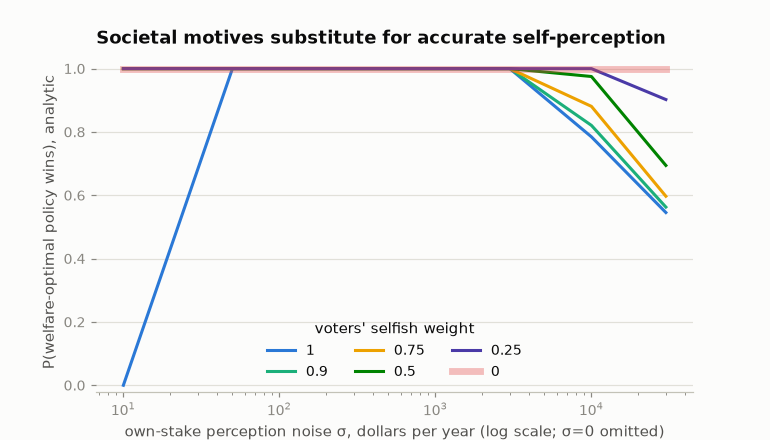
\includegraphics[width=.86\linewidth]{figures/mixed_motive_tracking.png}
\caption{Analytic tracking against own-stake noise by the voters'
selfish weight (informed societal component, 10{,}001 voters). Societal
motives substitute for accurate self-perception.}
\label{fig:mixed}
\end{figure}

\paragraph{Value pluralism is its own distortion channel.} Sociotropic
voting removes the misperception distortions and introduces one that no
perception survey can close: fully informed voters disagree because they
hold different welfare functions. On these policies the EDE ranking
flips between \(\eta = 2\) and \(\eta = 2.5\) --- at 2.5 the rate cap
edges the credit by all of \$2.88 per household (\(-\$696.74\) versus
\(-\$699.62\)). Split an all-informed sociotropic electorate between
\(\eta = 1\) and \(\eta = 2.5\) types and the outcome follows the
majority lens; graded against either welfare function, every majority
composition is simultaneously ``tracked'' under one and ``failed'' under
the other, and the 50/50 split is a coin flip under both.

\paragraph{A sociotropic minority disciplines candidates.} The
escalation of Section~\ref{sec:strategic} assumed every voter is a noisy
self-interested one. Mixing in a share \(q\) of informed sociotropic
voters (\(s = 0\), \(\eta = 1\)) against the same purely selfish
candidates dismantles it (Table~\ref{tab:discipline},
Figure~\ref{fig:discipline}). At \(q = 0.10\) every noise level has
pure equilibria again and all of them enact the status quo: the bloc
votes deterministically against whichever candidate proposes the more
welfare-negative program, and a tenth of the electorate outweighs the
selfish margin any program can buy among its beneficiaries. The
transition is not smooth: at \(q = 0.02\)--\(0.05\) and high \(\sigma\)
the pure-equilibrium set is \emph{empty} --- proposing a program wins
the noisy selfish margin until the opponent undercuts and takes the
sociotropic bloc, which restores the incentive to propose, and best
responses cycle with proposals reaching up to full intensity inside
the cycle. The bloc also degrades gracefully: sociotropic voters who misread
the societal value with \$500 of noise per household (against a signal
peaking near \$380) still cut enacted intensity at 30\% share from 0.65
to 0.11, while an electorate that is uniformly \emph{half} selfish ---
no informed bloc at all --- cuts it only from 0.63 to 0.44 on a
matched grid. A small bloc that votes the societal signal
deterministically disciplines far more than diffuse partial altruism,
which merely shrinks every voter's selfish margin.

\begin{table}[t]
\centering
\small
\begin{tabular}{lccc}
\toprule
Sociotropic share \(q\) & \(\sigma = \$1{,}000\) & \$10{,}000 & \$30{,}000 \\
\midrule
0 (baseline) & 0.19 & 0.65 & 0.55 \\
0.02 & cycling & cycling & cycling \\
0.05 & 0.00 & cycling & cycling \\
0.10--0.50 & 0.00 & 0.00 & 0.00 \\
\bottomrule
\end{tabular}
\caption{Mean enacted credit intensity across pure Nash equilibria,
purely selfish candidates. ``Cycling'' marks empty pure-equilibrium
sets, where best-response dynamics orbit instead; 0.00 is zero to
numerical precision.}
\label{tab:discipline}
\end{table}

\begin{figure}[t]
\centering
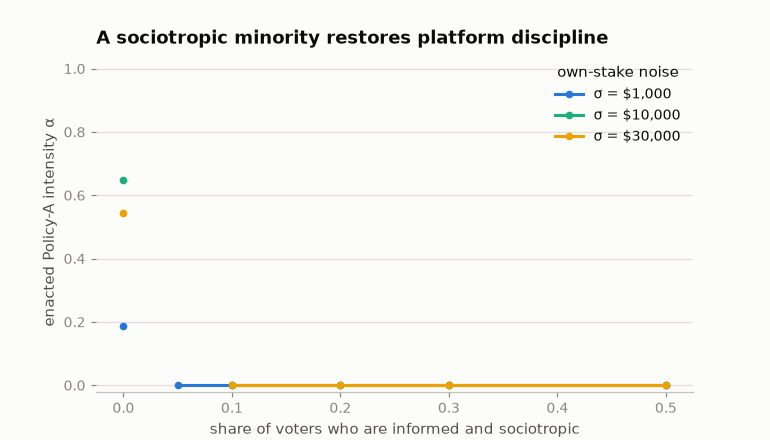
\includegraphics[width=.86\linewidth]{figures/strategic_discipline.png}
\caption{Enacted credit intensity against the informed-sociotropic voter
share, by own-stake noise. Gaps are the cycling regime of
Table~\ref{tab:discipline}.}
\label{fig:discipline}
\end{figure}

\section{A continuous axis: ideal outcomes and beliefs about policy}
\label{sec:axis}

Everything so far asks whether elections rank two policies correctly.
This section changes the object. The policy is a continuous dial;
voters care about the outcome the dial produces, not the dial; and what
they know is a belief about how far the dial moves the outcome. Demand
for policy is then derived, not primitive --- and wrong beliefs distort
it in a specific, measurable direction.

\paragraph{The dial.} A position \(t \in [0, 1]\) raises every federal
income tax bracket rate by \(10t\) percentage points and returns the
revenue as an equal per-adult transfer --- the
linear-tax-plus-demogrant axis of the redistribution literature, priced
on measured household incidence through the actual tax code. A
dedicated engine-built artifact (three simulations) carries it: at
\(t = 1\) the engine scores \$1{,}286.6B of revenue, a \$4{,}809
transfer per adult per year, and 68.6\% of households gaining net
(Table~\ref{tab:axis}); the Gini falls from 0.4541 to 0.4135 and EDE
income rises \$7{,}661 per household. Gross incidence interpolates
linearly in \(t\) from the endpoint run, and a midpoint engine run
prices the approximation: 0.31\% of totals, 97.4\% of households within
\$1, mean absolute error \$16.27. Mean net stake runs from
\(+\$7{,}777\) in the bottom income decile to \(-\$35{,}671\) in the
top and crosses in the eighth --- household size, not a single
break-even income, sets where the transfers stop covering the rate
increases.

\begin{table}[t]
\centering
\small
\begin{tabular}{lccc}
\toprule
Position & Gini & \(\Delta\)EDE per household & Transfer per adult \\
\midrule
\(t = 0\) (current law) & 0.4541 & --- & --- \\
\(t = 0.5\) & 0.4336 & \(+\$4{,}211\) & \$2{,}404 \\
\(t = 1\) & 0.4135 & \(+\$7{,}661\) & \$4{,}809 \\
\bottomrule
\end{tabular}
\caption{Measured outcomes along the redistribution axis. Position
\(t\) raises every federal bracket rate by \(10t\) points and returns
the revenue as an equal per-adult transfer; at \(t = 1\) the levy
raises \$1{,}286.6B and 68.6\% of households gain. A midpoint engine
run bounds the linear interpolation of gross incidence at 0.31\% of
totals, with 97.4\% of households within \$1.}
\label{tab:axis}
\end{table}

\paragraph{Preferences over outcomes, beliefs about the mapping.} A
voter holds an ideal Gini \(g^*_i\), a price \(k_i\) in dollars per
Gini point on missing it, and a selfish weight \(s_i\), on the same
dollar scale as the rest of the paper:
\begin{equation}
U_i(t) \;=\; s_i \cdot \widehat{\mathrm{own}}_i(t)
\;-\; (1 - s_i) \cdot k_i \cdot 100 \cdot
\bigl|\hat G_i(t) - g^*_i\bigr|.
\label{eq:axisutility}
\end{equation}
Beliefs enter as a slope on the outcome mapping, not as noise on each
option:
\begin{equation}
\hat G_i(t) \;=\; G(0) \;+\; \lambda_i \bigl(G(t) - G(0)\bigr),
\label{eq:axisbelief}
\end{equation}
with \(\lambda_i = 1\) correct and \(\lambda_i < 1\) understating the
policy's reach. Own-stake perception works the same way: the perceived
own stake is \(t \cdot (\mathrm{own}_i + \varepsilon_i)\) with one draw
per voter, so a voter's perceived utility curve stays coherent across
the whole continuum instead of jumping between neighboring positions as
per-option noise would force.

\paragraph{Wrong beliefs inflate demand reciprocally.} A voter's belief
reports the target only once the true Gini reaches
\(G(0) + (g^*_i - G(0))/\lambda_i\), and the measured Gini curve is
nearly linear in \(t\) (grid steps from \(-0.00104\) at the bottom of
the axis to \(-0.00099\) at the top), so demanded position scales as
\(1/\lambda\) until the axis saturates. For the target halfway to the
axis's floor, demanded \(t\) runs 0.250 at \(\lambda = 2\), 0.325 at
1.5, 0.500 at 1, 0.650 at 0.75, and the entire axis at
\(\lambda \le 0.5\). A voter who wants half the achievable inequality
reduction and believes policy half as effective as it is demands
everything the axis offers --- the maximalist's platform, held for the
opposite reason. Read as measurement, stated policy demand identifies
values only jointly with beliefs; ``what policy do you support?''
separates the two only if both are elicited.

\paragraph{Elections aggregate beliefs by median, not mean.} Give the
electorate one shared goal --- a target Gini of 0.4338, half the axis's
reach --- and split it between correct voters (\(\lambda = 1\)) and
attenuated ones (\(\lambda = 0.25\)), with two office-seeking
candidates playing the position game. Sweeping the attenuated share: at
0--0.4 the equilibrium enacts exactly 0.500, what a fully correct
electorate enacts, even though at 0.4 the electorate's mean belief
understates the policy's reach by 30\%; at 0.5 it enacts 0.750; from
0.6 on, the maximum. Independent misperception canceled on the
two-option ballot of Section~\ref{sec:knife}; on a continuum the median
belief rules and the mean is irrelevant --- same electorate, same
perception machinery, opposite aggregation. The equilibria themselves
are exactly Downsian: across all 30 (target, belief) cells the enacted
position equals the electorate's median ideal to grid precision
\citep{downs1957}.

\paragraph{Self-interest wants the corner.} A purely self-interested
electorate enacts \(t = 1\) at every own-stake noise level tested
(\$0, \$1{,}000, \$10{,}000): 68.6\% of households gain from the full
program, so the median voter does, and one noise draw on a perceived
gradient leaves most voters' signs in place. This is the demand side of
\citet{meltzer1981} running on measured incidence rather than a
stylized income distribution. Moderation on this axis comes from values
(an ideal short of maximum equality) or from beliefs (an overestimate
of policy's reach), not from self-interest.

The engine holds labor supply, avoidance, and growth fixed, so more
redistribution always raises EDE income and the inequality-averse
planner's optimum is the corner \(t = 1\); every interior result above
comes from voters' ideal points, not from an efficiency cost. This
section models demand formation, not optimal taxation. The target,
belief-slope, and price distributions are labeled assumptions --- the
survey targets --- and the belief slope is a single elicitable number:
what a respondent expects a ten-point rate rise returned as an equal
check to do to inequality.

\section{Robustness and limitations}\label{sec:limits}

The welfare ranking is stable across \(\eta \in \{0.5, 1, 2\}\) and under
per-capita and square-root equivalence scales, but flips to Policy B by
\(\eta = 2.5\) (holding at the higher tested values), where the
\$1{,}000 income floor's censoring of the
poorest households' levies dominates; the ranking is a modeling choice,
reported as such, and Section~\ref{sec:preferences} converts the
sensitivity into a mechanism. Both financing rules hand the no-stakes
bloc its signed sliver; financing choices that zero it, or deficit
financing that hides it, restore monotone tracking. Errors are
independent across voters --- including adults in the same household ---
and across policies; household-correlated error is not simulated here
and could change the levy bloc's effective behavior.

The endogenous layers carry their own scope. The position game is two
candidates, one shot, pure strategies on a grid, in the
two-dimensional space the measured incidence vectors span; mixed
strategies in the cycling regime are not computed (best-response
dynamics are reported instead), and entry, primaries, dynamics, and
commitment problems are out of scope. Voter types mix independently of
stakes and demographics; the societal signal a voter perceives is the
EDE change of the electorate actually voting; and the societal noise,
bias, and \(\eta\) distributions are labeled assumptions with nothing
measured behind them --- the layer exists so that survey estimates of
sociotropic perception can drop in beside the own-stake ones.

Ballots are sincere under every rule of Section~\ref{sec:rules}: score
voters spend the full scale or report clipped dollar values, approval
voters apply a fixed threshold, and nobody strategizes; strategic
exaggeration would push the cardinal rules toward approval, their
bracketing case. The rules comparison also fixes one agenda --- the
two measured programs plus the status quo --- and rule performance
under other agendas is untested. The axis of Section~\ref{sec:axis}
holds behavior fixed, so more redistribution always raises EDE income,
the inequality-averse planner's optimum sits at the corner, and every
interior result there comes from voters' ideal points rather than an
efficiency cost; its target, belief-slope, and price distributions are
labeled assumptions awaiting the same survey.

The binding limitation is that perception is assumed. The linear-Gaussian
family is exactly what a survey regression of perceived on true impacts
would estimate --- attenuation, bias, and residual dispersion, by
demographic cell --- and the model's perception interface accepts a fitted
empirical distribution without modification. Measured tax-policy knowledge, beliefs, and perceived distributional
effects exist in the literature \citep{bartels2005, stantcheva2021}, but
not the engine-computed, own-household incidence beliefs this model
consumes; eliciting it is the natural next
step, and its answer is a single point on the axes swept here.

\section{Conclusion}

On measured household stakes, the relationship between voter accuracy and
welfare tracking inverts the toy intuition at both ends: elections track
almost perfectly across two orders of magnitude of misperception, fail on
a welfare-irrelevant residual at perfect information unless the
trivial-stakes majority goes silent, scale their thresholds with
electorate size, and trade a thousand dollars of noise tolerance for a
two-hundred-dollar bias vulnerability. Making the platforms choices
flips the verdict on information: perfect information disciplines
competing candidates to the status quo --- here the welfare optimum ---
while the same noise that rescued fixed-platform tracking is what lets
self-serving programs through, eroding even the electoral advantage of
broad constituencies over narrow ones. And the cheapest repairs live in
preferences, not information: a few percent of utility weight on society
cures the knife-edge, and a tenth of the electorate voting an informed
societal signal disciplines purely selfish candidates at any noise
level, leaving value pluralism --- informed voters with different
inequality aversions --- as the distortion no measurement closes.
The wider objects sharpen both points. With the status quo votable,
every rule tested tracks perfectly at perfect information --- the
agenda, not the aggregation, made the knife-edge --- yet a one-word
approval convention swings that same outcome from 0\% to 100\%, noise
reverses the rule ordering, and no gap between rules approaches what
the ballot's option set decides. On a continuous redistribution axis
the aggregation itself flips: independent misperception stops
canceling, the median belief sets the outcome, demand for policy
inflates with the reciprocal of belief in its reach, and pure
self-interest rides measured incidence to the corner at every noise
level; moderation falls to values and beliefs. The mechanisms are old;
the denominations are new. Whether real electorates sit on the
tracking side of these numbers --- how accurately voters see their own
stakes, how far they believe policy moves the outcomes they value, how
much weight they place on society's, and through which welfare lens ---
is now a measurement question.

\begin{thebibliography}{18}
\itemsep2pt

\bibitem[Atkinson(1970)]{atkinson1970}
Atkinson, A.~B. (1970). On the measurement of inequality. \emph{Journal
of Economic Theory}, 2(3), 244--263.

\bibitem[Bartels(2005)]{bartels2005}
Bartels, L.~M. (2005). Homer gets a tax cut: Inequality and public policy
in the American mind. \emph{Perspectives on Politics}, 3(1), 15--31.

\bibitem[Besley and Coate(1997)]{besley1997}
Besley, T., and Coate, S. (1997). An economic model of representative
democracy. \emph{Quarterly Journal of Economics}, 112(1), 85--114.

\bibitem[Calvert(1985)]{calvert1985}
Calvert, R.~L. (1985). Robustness of the multidimensional voting model:
Candidate motivations, uncertainty, and convergence. \emph{American
Journal of Political Science}, 29(1), 69--95.

\bibitem[Caplan(2007)]{caplan2007}
Caplan, B. (2007). \emph{The Myth of the Rational Voter: Why Democracies
Choose Bad Policies}. Princeton University Press.

\bibitem[Condorcet(1785)]{condorcet1785}
Condorcet, M.~J.~A.~N. de Caritat, Marquis de (1785). \emph{Essai sur
l'application de l'analyse \`a la probabilit\'e des d\'ecisions rendues
\`a la pluralit\'e des voix}. Paris.

\bibitem[Coughlin and Nitzan(1981)]{coughlin1981}
Coughlin, P., and Nitzan, S. (1981). Electoral outcomes with probabilistic
voting and Nash social welfare maxima. \emph{Journal of Public Economics},
15(1), 113--121.

\bibitem[Dahl(1956)]{dahl1956}
Dahl, R.~A. (1956). \emph{A Preface to Democratic Theory}. University of
Chicago Press.

\bibitem[Downs(1957)]{downs1957}
Downs, A. (1957). \emph{An Economic Theory of Democracy}. Harper.

\bibitem[Edlin et~al.(2007)]{edlin2007}
Edlin, A., Gelman, A., and Kaplan, N. (2007). Voting as a rational
choice: Why and how people vote to improve the well-being of others.
\emph{Rationality and Society}, 19(3), 293--314.

\bibitem[Feddersen and Pesendorfer(1996)]{feddersen1996}
Feddersen, T., and Pesendorfer, W. (1996). The swing voter's curse.
\emph{American Economic Review}, 86(3), 408--424.

\bibitem[Kinder and Kiewiet(1981)]{kinder1981}
Kinder, D.~R., and Kiewiet, D.~R. (1981). Sociotropic politics: The
American case. \emph{British Journal of Political Science}, 11(2),
129--161.

\bibitem[Ladha(1992)]{ladha1992}
Ladha, K.~K. (1992). The Condorcet jury theorem, free speech, and
correlated votes. \emph{American Journal of Political Science}, 36(3),
617--634.

\bibitem[Lindbeck and Weibull(1987)]{lindbeck1987}
Lindbeck, A., and Weibull, J.~W. (1987). Balanced-budget redistribution as
the outcome of political competition. \emph{Public Choice}, 52(3),
273--297.

\bibitem[Meltzer and Richard(1981)]{meltzer1981}
Meltzer, A.~H., and Richard, S.~F. (1981). A rational theory of the
size of government. \emph{Journal of Political Economy}, 89(5),
914--927.

\bibitem[Osborne and Slivinski(1996)]{osborne1996}
Osborne, M.~J., and Slivinski, A. (1996). A model of political
competition with citizen-candidates. \emph{Quarterly Journal of
Economics}, 111(1), 65--96.

\bibitem[Page and Shapiro(1992)]{page1992}
Page, B.~I., and Shapiro, R.~Y. (1992). \emph{The Rational Public: Fifty
Years of Trends in Americans' Policy Preferences}. University of Chicago
Press.

\bibitem[Stantcheva(2021)]{stantcheva2021}
Stantcheva, S. (2021). Understanding tax policy: How do people reason?
\emph{Quarterly Journal of Economics}, 136(4), 2309--2369.

\bibitem[Wittman(1983)]{wittman1983}
Wittman, D. (1983). Candidate motivation: A synthesis of alternative
theories. \emph{American Political Science Review}, 77(1), 142--157.

\end{thebibliography}

\end{document}
